\section{Machine Learning Model Introduction}
In our project, we will use a Multi-layer Perceptron Neural Network to price an option. 
\subsection{Neural Network}
At their core, neural networks work by imitating the neurons in our brains to try and make predictions or classifications. The most popular neural network used to predict numerical data is a multi-layer perceptron (MLP) which works by receiving independent input into a few nodes, passing the data through a series of hidden layers of neurons, and predicting an output. Based on the accuracy of the output, the weight given to each neuron changes and the model runs again until it reaches an optimal value. 

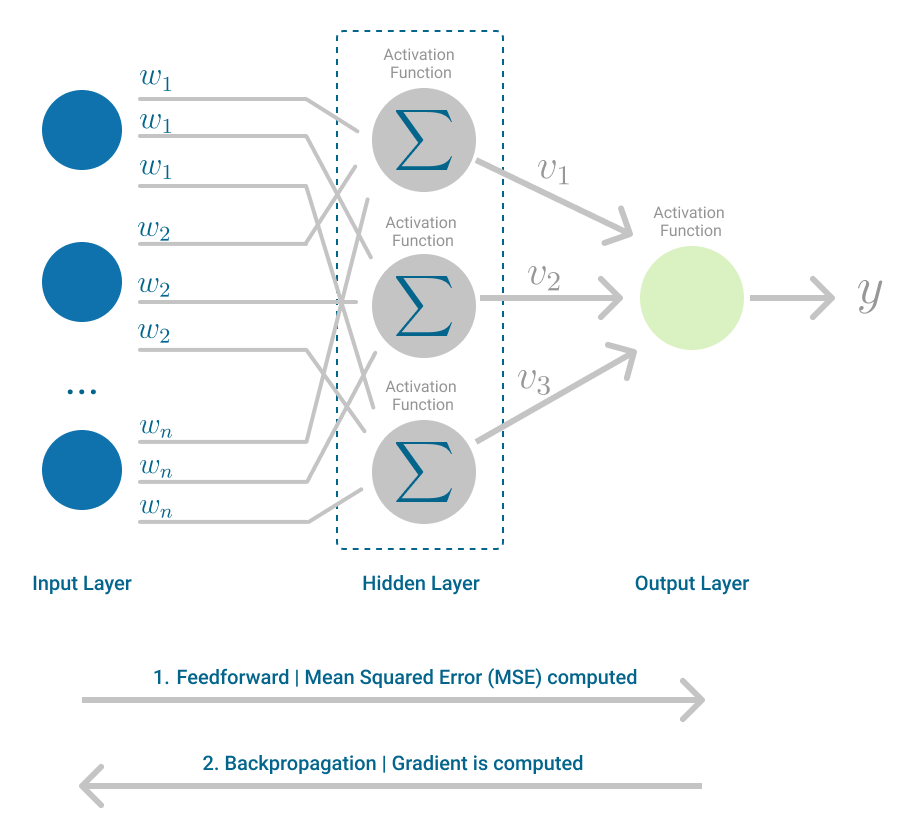
\includegraphics[width=.5\textwidth]{graphics/MLNNGraphic.png}
\\
As can be seen from the above image, the model works by taking a set of numerical inputs, multiplying each by a weight which is then passed through a nonlinear activation function in the first hidden layer. Note that if the activation function is linear, this MLP would work like a multiple linear regression or logistic regression. These activation functions then run and take on weights of their own, which then get passed on to other hidden layers. Once the output is calculated, it is compared to the expected output and the weights are tuned to minimize the model’s loss function or the distance between the model's output and the expected output. This optimization happens through gradient descent or an improved version of it. After the MLP has trained for enough time, it converges to a local minimum, and the model is considered trained. MLP models have been extensively used to model financial data and make predictions based on numerical values. We use a stock option’s strike price, current price, time until expiration, interest rate, and historical volatility in order to predict the best value for the stock option. \cite{MLIntro}

\subsection{Root Mean Squared Error}
Root Mean Squared Error (RMSE) is calculated to be the standard deviation of the prediction errors (otherwise known as \textit{residuals}. It can be more specifically described as the square root of the mean of the square of the errors. In machine learning, RMSE is used to measure how accurate the set of predictions from a model is. \cite{RMSE}
$$RMSE = \sqrt{\frac{1}{n}\sum_{i=1}^n S_i - {O_i}^2}$$
Where 
$$n = number\; of \; observations$$
$${O_i}^2 = observed\; value$$
$$S_i = predicted \; values$$
% \subsection{Yang-Zhang Volatility Model}
